%% ELEC2013 2007

%% ----------------------------------------------------------------
%% exam.tex
%% ----------------------------------------------------------------
\documentclass{sotonExamBoxes}    % use option [answers] to include them
%\documentclass[answers]{uosexamb}
%% ----------------------------------------------------------------
\usepackage{graphicx}
%\usepackage{pstricks}
\usepackage{alltt}
\usepackage{bm}
\usepackage{amssymb}
\usepackage{amsfonts}
\usepackage{amsmath}
\thinmuskip=1mu
%\renewcommand{\ttdefault}{pcr}
\renewcommand{\ttdefault}{pcr}
\newcommand{\tr}{\textsf{T}}
\newcommand{\e}[1]{{\rm e}^{#1}}
\newcommand{\E}[1]{{\rm e}^{{\displaystyle #1}}}
\newcommand{\logg}[1]{\log\left(#1\right)}
\newcommand{\bra}[1]{\left(#1\right)}
\newcommand{\Prob}[1]{\mathbb{P}\left(#1\right)}
\newcommand{\Step}{\mathop{\mathrm{O}\hspace{-15pt}\rule[8.5pt]{11pt}{1.2pt}\hspace{2pt}}}
\newcommand\diag{\mathop{\mathrm{diag}}}
\newcommand{\grad}{\bm{\nabla}}
\newcommand{\dd}{\mathrm{d}}
\newcommand{\class}{\mathcal{C}}
\newcommand{\data}{\mathcal{D}}
\DeclareMathAlphabet{\mat}{OT1}{cmss}{bx}{n}
\newcommand{\pd}[2]{\ensuremath{\frac{\partial #1}{\partial #2}}\xspace}
\newcommand{\M}[1]{\ensuremath{\boldsymbol{#1}}\xspace}
\newcommand{\bst}{\rule{0mm}{5mm}}
\newcommand{\av}[2][\,]{\mathbb{E}_{#1}\!\left[ {\strut #2} \right]}
\newcommand{\len}[1]{\| #1 \|}
\graphicspath{{figures/} {../2018-19/figures}}
\newcommand{\inner}[2]{\left\langle #1, #2\right\rangle}
\graphicspath{{figures/}}
\newcommand{\squeeze}{\setlength{\itemsep}{-2pt}}
\newcommand{\Tr}{\mathop{\mathrm{tr}}\,}

% \usepackage{picture}
\begin{document}
\unitTitle{Problem Sheet 2 for Advanced Machine Learning (COMP6208)}
\authors{Adam Pr\"ugel-Bennett}
\unitcode{COMP6208}
\semester{2}
\year{2022}
\duration{45}{0}


\maketitle


%\blankpage


%% ----------------------------------------------------------------
%\section
% -----------------------------------------------------------------------
% *************************  Section A  *********************************
% -----------------------------------------------------------------------

% ***************************** question 1 **************************



\begin{question}{15}
  \begin{qparts}
    \qpart[2]{To find the minimum of a 1-d function,  we can do an iterative
       update
       \begin{align*}
         x^{(t+1)} =x^{(t)} - r\, f'(x^{(t)})
       \end{align*}
       where $r$ is a learning rate and $f'(t)$ is the  derivative of
       the function, $f(x)$ we are minimising.  Supposing that
       \begin{align*}
         f(x) = \frac{c}{2} (x-x^*)^2
       \end{align*}
       where $c>0$.  Write down a recursion formula for $x^{(t+1)}$ and
       $x^{(t)}$.}{\lines{2}}
      \begin{answer}
        \begin{align*}
          x^{(t+1)} &=x^{(t)} - c\,r\,(x^{(t)}-x^*) \\
                      &=(1-c\,r) x^{(t)} + c\,r\,x^*.
        \end{align*}
      \end{answer}
      \qpart[5]{Show by induction that
        $x^{(t)} = F(t) = x^* + (x^{(0)}-x^*)\,(1-c\,r)^t$ is a solution
        to the recursion relation.  Hence find a condition on the
        value of $r$ to ensure convergence.}{\lines{12}}
      \begin{answer}
        In the base case, if we take $t=0$ then
        \begin{align*}
          F(0) &= x^* + (x^{(0)}-x^*)\,(1-c\,r)^0 \\
          &= x^* + (x^{(0)}-x^*) = x^{(0)}.
        \end{align*}
        Thus the formula is true for $t=0$.  Assuming the formula is
        true for $x^{(t)}$ then substituting this into the recursion
        relation
        \begin{align*}
          x^{(t+1)} &=(1-c\,r) F(t) + c\,r\,x^*\\
          &= (1-c\,r) \bra{x^* + (x^{(0)}-x^*)(1-c\,r)^t} +
                      c\,r\,x^* \\
          &= x^* + (x^{(0)}-x^*)(1-c\,r)^{(t+1)} = F(t+1).
        \end{align*}
        Thus, we shown that assuming $x^{(t)} = F(t)$ then $x^{(t+1)}
        = F(t+1)$, but as it is true for $t=0$ the formula will be
        true for all non-negative integers.

        The condition for convergence is that $0<c\,r<2$.  Assuming
        $c>0$ then $0<r<2/c$.
      \end{answer}
      \qpart[2]{
        Now consider the case when $\bm{x}\in\mathbb{R}^n$.  We assume
        that
        \begin{align*}
          g(\bm{x}) = \frac{1}{2} (\bm{x} - \bm{x}^*)^\tr \mat{Q} \,(\bm{x} - \bm{x}^*)
        \end{align*}
        where $\mat{Q}$ is a symmetric, positive-definite matrix.
        The Hessian, $\mat{H}$, of $g(\bm{x})$ is a matrix with
        components
        \begin{align*}
          H_{ij} = \frac{\partial^2 g(\bm{x})}{\partial x_i\, \partial x_j}.
        \end{align*}
        By writing out $g(\bm{x})$ as a double sum over the components
        compute the Hessian
      }{\lines{8}}
      \begin{answer}
        \begin{align*}
          H_{ij} = \frac{\partial^2 \hspace{5mm}}{\partial x_i\,
          \partial x_j}\, \frac{1}{2} \sum_{k\,\ell} (x_k-x^*_k)
          Q_{k\ell} (x_\ell-x^*_\ell) = Q_{ij} 
        \end{align*}
      \end{answer}
      \qpart[2]{Gradient descent in $\mathbb{R}^n$ is given by
        \begin{align*}
                  \bm{x}^{(t+1)} = \bm{x}^{(t)} -r\, \grad g(\bm{x}) .
        \end{align*}
        Using the definition of $g(\bm{x})$ write down a recursion
        relation between $\bm{x}^{(t+1)}$ and $\bm{x}^{(t)}$.
      }{\lines{2}}
      \begin{answer}
        \begin{align*}
          \bm{x}^{(t+1)} = \bm{x}^{(t)} - r \, \mat{Q}\, (\bm{x}^{t} -
          \bm{x}^*)
        \end{align*}
      \end{answer}
      \qpart[2]{Defining $\bm{\Delta}^{(t)}=(\bm{x}^{(t)} - \bm{x}^*)$
        obtain a recursion relation between $\bm{\Delta}^{(t+1)}$ and
        $\bm{\Delta}^{(t)}$. (This is easy if you subtract $\bm{x}^*$
        from both sides of the recursion equation for
        $\bm{x}^{(t+1)}$.)}{\lines{2}}
      \begin{answer}
        \begin{align*}
          \bm{\Delta}^{(t+1)} = (\mat{I}- r \, \mat{Q}) \, \bm{\Delta}^{(t)}.
        \end{align*}
      \end{answer}
      \qpart[3]{Using the eigenvalue decomposition $\mat{Q} =
        \mat{V}\,\mat{\Lambda}\,\mat{V}^\tr$ and defining
        $\bm{z}^{(t)} = \mat{V}^\tr \bm{\Delta}^{t}$ write out a
        recursion relation between $\bm{z}^{(t+1)}$ and
        $\bm{z}^{(t)}$. (This is helped by multiplying the recursion
        relation on the left by $\mat{V}^\tr$ and using the fact that
        $\mat{V}$ is an orthogonal matrix.)}{\lines{4}}
      \begin{answer}
        \begin{align*}
          \bm{z}^{(t+1)} = (\mat{I} - r \mat{\Lambda}) \bm{z}^{t}
        \end{align*}
      \end{answer}
      \qpart[4]{Solve the recursion relation to obtain a formula for
        $\bm{x}^{(t)}$ in terms of the initial state $\bm{x}^{(0)}$.
        Express this formula for the $i^{th}$
        component of $\bm{x}^{(t)}$ and hence find a condition on the
        learning rate $r$ to ensure convergence.}{\lines{8}}
      \begin{answer}
        The solution to the recursion equation is trivially.
        \begin{align*}
          \bm{z}^{(t)} = (\mat{I} - r \mat{\Lambda})^t \bm{z}^{(0)}.
        \end{align*}
        As $\mat{\Lambda}$ is diagonal
        \begin{align*}
          z_i^{(t)} = (1-r\,\lambda_i)^t\, z_i^{(0)}.
        \end{align*}
        Thus the condition for $z_i^{(t)}$ to converge is that
        $0<r\,\lambda_i<2$.  For all $\bm{z}^{(t)}$ to converge we
        require $0<r<2/\lambda_{max}$.
      \end{answer}
  \end{qparts}
\end{question}
\freshpage

% ***************************** question 2 **************************

\begin{question}{15}
  \begin{qparts}
    \qpart[5]{Consider the non-quadratic minimum at $x^*$ given by
      \begin{align*}
        f(x) = \frac{c}{2} \,(x-x^*)^2 + \frac{d}{6}   \,(x-x^*)^3
      \end{align*}
      where we use Newton's method
      \begin{align*}
        x^{(t+1)} = x^{(t)} - \frac{f'(x^{(t)})}{f''(x^{(t)})}.
      \end{align*}
      by computing the derivatives and expanding for small
      $x^{(t)}-x^{*}$ show that\\
      $x^{(t+1)}-x^{*} = O\bra{\bra{x^{(t)}-x^{*}}^2}$ .

      (To do this we need to expand a term with the structure
      \begin{align*}
        \frac{r + s \, \epsilon}{u + v \,\epsilon}.
      \end{align*}
      Note that we can use the geometric series expansion to write
      \begin{align*}
         \frac{1}{u + v \,\epsilon} = \frac{1}{u} \frac{1}{1
        +\frac{v}{u} \epsilon} = \frac{1}{u} \bra{1 - \frac{v}{u}\epsilon +
        \bra{\tfrac{v}{u}\epsilon}^2 - \cdots}
      \end{align*}
      which is convergent provided $|\tfrac{v}{u}\epsilon|<1$.
      )
    }{\lines{10}}
    \begin{answer}
      Using
      \begin{align*}
        f'(x) &= c\,\bra{x-x^{*}} + \frac{d}{2} \, \bra{x-x^{*}}^2
                &
        f''(x) &= c + d \, \bra{x-x^{*}}
      \end{align*}
      so that
      \begin{align*}
        x^{(t+1)} = x^{(t)} - \frac{c\,\bra{x^{(t)}-x^{*}} +
        \frac{d}{2} \, \bra{x^{(t)}-x^{*}}^2}{c + d \,
        \bra{x^{(t)}-x^{*}}}
      \end{align*}
      Subtracting $x^{*}$ from both sides of this equation and
      writing $\epsilon^{(n)} = x^{(t)}-x^{*}$.  We find
      \begin{align*}
        \epsilon^{(t+1)}
        &= \epsilon^{(t)} - \frac{c\,\epsilon^{(t)} +
        \frac{d}{2} \, \bra{\epsilon^{(t)}}^2}{c + d \,\epsilon^{(t)}}
        \\
        &=  \epsilon^{(t)}  - \bra{c\,\epsilon^{(t)} +\frac{d}{2}\bra{\epsilon^{(t)}}^2}
        \frac{1}{c} \bra{1 - \frac{d}{c}  \epsilon^{(t)} +
          \frac{d^2}{c^2}  \bra{\epsilon^{(t)}}^2 + \cdots}
        \\
        &= \frac{d}{2\,c}   \bra{\epsilon^{(t)}}^2  +
          O\bra{\bra{\epsilon^{(t)}}^3}
          = O\bra{\bra{\epsilon^{(t)}}^2}
      \end{align*}
      that is $x^{(t+1)}-x^{*} = O\bra{\bra{x^{(t)}-x^{*}}^2}$.
    \end{answer}
    \freshpage
    \qpart[2]{Consider the function
      \begin{align*}
        h(x) = - x\, \log(x)
      \end{align*}
      defined for $0<x\leq 1$.  By computing $h'(x)$ and setting
      $h'(x)=0$ compute the value of $x^*$ that maximises $h(x)$.
    }{\lines{5}}
    \begin{answer}
      \begin{align*}
        h'(x) = - \log(x) -1
      \end{align*}
      Thus $h'(x) = 0$ has a solution at $x^* = \e{-1}$.
    \end{answer}
    \qpart[3]{Compute $h''(x)$ and thus compute the Newton update
      function
      \begin{align*}
        n(x) = x - \frac{h'(x)}{h''(x)}
      \end{align*}
      (the answer is rather surprising and in no way general).}{\lines{5}}
    \begin{answer}
      $h''(x) = \tfrac{-1}{t}$ so that
      \begin{align*}
        n(x) =  x - x\,\bra{x\,\log(x)+1} =  -x\,\log(x).
      \end{align*}
      It is a coincident that $n(x) = h(x)$.
    \end{answer}
    \freshpage
    \qpart[10]{On the axes given below plot $x^{(t)}$ for $t=0,1,2,\ldots,10$,
      starting from $x^{(0)}=0.5$ where we use the gradient ascent updates
      \begin{align*}
        x^{(t+1)} = x^{(t)} + r\, h'(x^{t})
      \end{align*}
      for $r=\{0.3, 0.4, 0.5\}$ (that is you should plot three curves).

      Also plot $x^{(t)}$ where $x^{(t+1)} = n(x^{(t)})$ (that is
      using Newton's update formula) for $t=0, 1, 2, 3$ and
      $4$---note that to machine precision $x^{(5)}=x^*$.
    }{\qfig[0.9\linewidth]{convergence_q}}
    \begin{answer}
      \begin{center}
        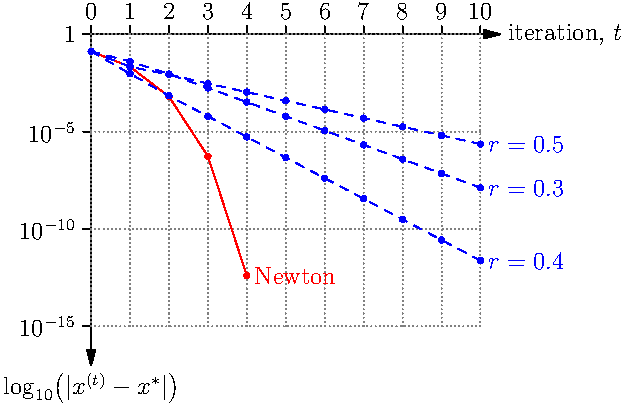
\includegraphics[width=0.9\linewidth]{convergence_a}
      \end{center}
    \end{answer}
  \end{qparts}
\end{question}
\freshpage

\begin{question}{10}
  \begin{qparts}
    \qpart[3]{Show that for $p_i>0$ the function
      \begin{align*}
        h(\bm{p}) = - \sum_i p_i\,\log(p_i)
      \end{align*}
      is strongly convex-down.  Hint: show that the Hessian matrix is
      negative-definite.
    }{\lines{8}}
    \begin{answer}
      We note that the Hessian $\mat{H}$ has entries
      \begin{align*}
        H_{ij}
        &= \frac{\partial^2 h(\bm{p})}{\partial p_i \partial p_j} = 0
        & H_{ii} &= \frac{\partial^2 h(\bm{p})}{\partial p_i^2} 
                 = - \frac{1}{p_i}
      \end{align*}
      Thus the Hessian is a diagonal matrix with $H_{ii} = -1/p_i <0$
      (since $p_i>0$).  The eigenvalues of a diagonal matrix are equal
      to the diagonal elements so that $\lambda_i<0$ for all $i$.
      This is a necessary and sufficient condition for $\mat{H}$ to be
      negative-definite and hence $h(\bm{p})$ is strongly convex-down.
    \end{answer}
    \vspace{1cm}

    \qpart[2]{Write down the Lagrangian, $\mathcal{L}$, for the problem of maximising
      $h(\bm{p})$ subject to the constraints
      \begin{align*}
        \sum_i p_i &=1  & \sum_i p_i \,E_i = U.
      \end{align*}
      Then explain why there is a unique solution to this constrained
      optimisation problem.}{\lines{7}}
    \begin{answer}
      The Lagrangian is given by
      \begin{align*}
        \mathcal{L} = h(\bm{p}) - \alpha \bra{\sum_i p_i  -1}
        - \beta \, \bra{\sum_i p_i  \, E_i - U}.
      \end{align*}
      The problem has a unique solution because the Lagrangian is
      strongly convex-down.  This follows because $h(\bm{p})$ is
      strongly convex-down and the constraints are linear (both
      convex-up and convex-down).  The sum of a strongly convex
      function and another convex functions is strongly convex.
    \end{answer}
    \freshpage
    
    \qpart[5]{By setting $\partial \mathcal{L}/\partial p_i=0$ find the
      value of $p_i$ that maximises $\mathcal{L}$ in terms of $E_i$
      and the Lagrange multipliers. 
      Use the constraint $\sum_i p_i =1$ to eliminate the
      Lagrange multiplier that enforces this constraint.}{\lines{15}}
    \begin{answer}
      We note that
      \begin{align*}
        \frac{\partial h(\bm{p})}{\partial p_i} = -\log(p_i) -1 - \alpha
      -\beta E_i
      \end{align*}
      so that
      \begin{align*}
        p_i = \e{-\alpha -1 - \beta\,E_i}
      \end{align*}
      Using the constraint $\sum_i p_i =1$ then
      \begin{align*}
        \sum_i \e{-\alpha -1 - \beta\,E_i} =1
      \end{align*}
      Dividing through by this we find
      \begin{align*}
        p_i = \frac{\e{-\beta\,E_i}}{\sum_j \e{-\beta\,E_j}}.
      \end{align*}
      This is the famous Boltzmann distribution.
    \end{answer}
  \end{qparts}
\end{question}

\end{document}
